\documentclass[11pt]{article}
\usepackage{trishnote}
\usepackage{tgpagella}  % for sample text

\titles{First properties of intersection homology}
\author{ \textsc{Trishan Mondal} \\[0.15cm]
  \href{https://www.isibang.ac.in}{Indian Statistical Institute, Bangalore}}
\date{}

\begin{document}
\maketitle 

\begin{abstract}
    \noindent In this talk, we will discuss the homological properties of intersection homology like pushforward maps, excision and Mayer-Vietoris. We will compute the intersection homology of cones. We then discuss Whitney stratifications for complex quasi-projective varieties and the associated pseudomanifold structure on their underlying topological space. We will conclude with a discussion of Poincaré duality, Lefschetz hyperplane and hard Lefschetz theorems in the context of intersection homology. Main references \cite{maxim2019intersection}, \cite{kirwan2006introduction}.
\end{abstract}

\section{Functoriality of Intersection Homology}

\noindent In the last talk we have seen the definition of Intersection Homology, including some examples. Now we want to see how different Intersection homology theory is from ordinary homology theory. In order to see this we will begin with `functoriality'. Suppose we have a continuous map $f:X\to Y$. Does it naturlly induce a map $f_{\ast} : I^{p}S_{\ast}(X)\to I^{q}S_{\ast}(Y)$ in `intersection chain complexes'? where $p$ and $q$ are different perversity (GM) for the spaces $X$ and $Y$. For any $\sigma \in I^pS_{i}(X)$ we expect $f \circ \sigma \in I^qS_i(Y)$. We will see with an example, it is not the case. What can go wrong? 

\begin{itemize}
    \item[] Filtration of $X$ and $Y$ could be arbitraty and perversity depends on filtration, so does $\bar{p}$-allowable chains. For \textbf{example}, consider the space $X = \qty{\text{pt}}$ with natural stratification and $Y$ is a stratified space. $f:X \to Y$ be a continuous map. We have $IS_i(X)=S_i(X)$ and $f(\sigma)$ will be allowable with respect to $S$ if, $i \leq i -\codim (S) + \bar{q}(S)$. But for GM perversity it is not possible. 
\end{itemize}

\noindent There is one more problem. We know ordinary homology theory is homotopy invariant but Intersection Homology is not a homotopy invariant. We will shortly see a result regarding Intersection homology of open cone of compact manifold. We know open cone over any sapce is contractible  but the Intersection homology of open cone is not same as Intersection homology of point. One more constrcutive example. 

\begin{itemize}
    \item[] \textbf{Example -- } Let, $X = \s^4 \vee \s^4$ and $Y = \s^4 \cup_{\C P^1 } \C P^2$. Now if we look at the inclusion $\C P^1 \hookrightarrow \C P^2$, it is a cofibration. Thus if we contract $\C P^1$ in $Y$ we will get, $\s^4 \vee \s^4 = X$. So, $X$ and $Y$ is homotopy equaivalent. But from talk $3$ we know, \begin{align*}
        I^{p}H_{k}(X) = \begin{cases}
            \F \oplus \F  & \text{ for } k = 0,4 \\
            0 & \text{otherwise}
        \end{cases}
    \end{align*}
    Again normalizaion of the space $Y$ is $\s^4 \sqcup \C P^2$. Both $\s^4$ and $\C P^2$ are manifold, so $IH_{\ast}(Y) \cong H_{\ast}(Y)$. For index $2$ we will have the intersection homology group as $\F$, which doesn't match with intersection homology group of $X$.
\end{itemize}

\noindent To resolve the issue we will define a special class of map between stratified space so that it will naturally induce map in intersection chain complexes. Thus we will come up with the following definitions. 

\begin{Def}{(Stratum-Preserving map)}{}
     A continuous map between startified spaces, $f : X \to Y$ is called startum preserving, if for each stratum $T$ of $Y$, the inverse image $f^{-1}(T)$ is union of strata of $X$. Equivalently image $f(S)$ is contained in a single starta of $Y$.
\end{Def}

\begin{Def}{($(\bar{p},\bar{q})$-stratified map)}{}
    A stratum preserving map $f : X \to Y$ is said to be $(\bar{p},\bar{q})$-stratum preserving if for any stratum $S\subset X$ contained in startum $T \subset Y$ satisfying , $$\bar{p}(S)-\codim_X(S) \leq \bar{q}(T) - \codim_{Y}(T)$$
\end{Def}

\noindent \textbf{Example \textcolor{darkcerulean}{1.1} -- } Let, $Y = X\times I$ be the space where $X$ comes with it's stratifications and $I$ is trivially filtered. The strata of $Y$ have form $S \times I$ where $S$ is a strata of $X$. The codimension of $S$ in $X$ is equal to codimension of $S \times I$ in $Y$. Let's take the perversity $q(S\times I) = p(S)$. Let, $f : X \to X \times I$ be the inclusion $x \mapsto (x,i_0)$. Then $f$ is $(p,q)$-stratified.

\vspace*{0.2cm}

\noindent \examp{1.2} (\textit{Placid Maps}) A stratified map $f : X \to Y$ is called placid if for ecah stratum $T\subset Y$ we have $\codim_Y(T) \leq\codim_X(f^{-1}(T))$. Now any placid map is a $(p,p)$-stratified map (using growth conditions of GM perversity).

\vspace*{0.2cm}

\prop{1.1} If $X$ and $Y$ are filtered space and $f : X \to Y$ is $(p,q)$-stratified then $f$ induces a map of intersection chain complexes (singular) $f_{\ast} : I^pS_{\ast}(X) \to I^qS_{\ast}(Y)$. 

\vspace*{0.2cm}

\noindent \textit{proof.} If $\sigma : \D^i \to X$ is a $p$-allowable simplex then for composition $f \circ \sigma$ we must consider $(f\sigma)^{-1}(T) = \sigma^{-1}f^{-1}(T)$ for singular strata of $Y$. Now, \[\sigma^{-1}f^{-1}(T) \subset \bigcup_{S : f(S)\subset T}\sigma^{-1}(S)\] For each such $S$ we have, \begin{align*}
    \sigma^{-1}(S) & \subset \qty{i - \codim(S) + p(S)}-\text{skeleta of } \D^i \\
    & \subset \qty{i - \codim(T) + q(T)}-\text{skeleta of } \D^i
\end{align*} Thus $f\circ \sigma$ is $q$-allowable. Thus we get a map $f_{\ast}: I^pS_{\ast}(X) \to I^qS_{\ast}(Y)$. $\hfill \blacksquare$

\vspace*{0.2cm}

\noindent Now we note that, this map is natural i.e. the following diagram commutes , \[\begin{tikzcd}
    {I^pS_i(X)} & {I^qS_i(Y)} \\
    {I^pS_{i-1}(X)} & {I^qS_{i-1}(Y)}
    \arrow["{\p_i^X}"', from=1-1, to=2-1]
    \arrow["{\p_i^Y}", from=1-2, to=2-2]
    \arrow["{f_{\ast}}", from=1-1, to=1-2]
    \arrow["{f_{\ast}}"', from=2-1, to=2-2]
    \end{tikzcd}\] So, cycle maps to cycle and boundary goes to boundary, in other words $f$ induce a map is Intersection homology groups $f_{\ast}: I^pH_{\bullet}(X) \to I^qH_{\bullet}(Y)$. Just for technicality we must mark this result that, a placid  map $f$, induce $f_{\ast}:I^pH_{\bullet}(X) \to I^pH_{\bullet}(Y)$. As a corollary to the previous proposition we can say, 

    \coro{ If $f$ is a startified homeomorphism and the perversities of $X$ corespond a perversity $q$ on $Y$ (i.e. $p(S)=q(T)$ if $f(S)=T$), then $I^pH_{\ast}(X) \simeq I^qH_{\ast}(Y)$.}

    \noindent Now we will strenthen the conditions on the map so that we can obtain a version of homotopy invariance for intersection homology.

    \begin{Def}{(Codimension Preserving)}{}
        A stratum preserving map is codimension preserving, if for each stratum $T$ of $Y$ we have $$\codim_YT =\codim_Xf^{-1}(T)$$
    \end{Def}

  \noindent As an \textbf{Example} we can note, the map $f : X \to X \times I$ by $x \mapsto (x,i_0)$ is codimension preserving. With this we are ready to define stratum-preserving homotopy equivalance.

  \begin{Def}{(Stratified Homotopic maps)}{}
     Let, $X,Y$ are filtered spaces with perversities $p,q$ and $X\times I$ has product filtration (as we discussed above) and by abuse of notation $p(S)=p(S \times I)$. Two codimension preserving map $f$ and $g$ from $X$ to $Y$ are homotopic if, there is a codimension preserving map $$H : X \times I \to Y$$ with $f = H|_{X\times \qty{0}}$ and $g= H|_{X \times \qty{1}}$.

     \vspace*{0.2cm}

     \noindent A \textbf{stratum preserving homotopy equivalance} between pseudomanifold $X$ and $Y$ is a pair of codimension preserving map $f: X \to Y$ and $g:Y \to X$  so that $f \circ g $ and $g \circ f$ are homotopic via stratified homotopies, $$H : X \times I \to X \, \text{ and } K: Y \times I \to Y$$
  \end{Def}

  \begin{Thm}{Friedman \cite{Friedman_2003}}{}
          If $f$ is a stratum-preserving homotopy equivalance, then the natural map $$f_{\ast}:I^pH_i(X) \xrightarrow{\simeq} I^pH_i(Y)$$
  \end{Thm}

  \noindent (\textbf{Kunneth}) As an application to the theorem we can say, the inclusion $X \hookrightarrow X \times (0,1)$ is a stratum preserving homotopy equivalance. Thus for a perversity $p$ we must have, \[\text{  }  I^pH_i(X) \simeq I^pH_i(X\times (0,1))\] \textsc{Remark:} \textit{All the definition above depends on a stratification of the space. We could re write the definitions conditionally. For example the definition of placid maps. We will prove that intersection homology is a topological invariant using sheaf theoretic intersection homology. This in particularlly means intersection homology is independent of startification.}

  \section{Relative Intersection Homology and Mayer-Vietoris sequences}

  Recall. For a topological space $X$ and $Y \subset X$, the relative chain complex $S_i(X,Y) = S_i(X)/S_i(Y)$ makes sense. Thus we can define relative homology groups easily. But for intersection homology there is a problem of defining the quotient $I^pS_i(X)/I^pS_i(Y)$. 
  \begin{itemize}
    \item[] The problem in this case is that, $p$-allowable chains of $Y$ depends on the filtration of $Y$ which might not be related to the startification of $X$. For \textbf{Example}, $X$ be a stratified space with a perversity $p$ and $Y =\qty{x}$ is a subspace of $X$. For $Y$, the filtration should be same as a $0$-dim manifold. And $\qty{x}$ is the only regular starta of $Y$. So for any perversity $p$, $p(\qty{x})=0$. So, $I^pS_{\ast}(Y) = S_{\ast}(Y)$. If $Y$ was in the singular starta of $X$, the intersection chains of $X$ can't pass through $\qty{x}=Y$. Then we will not have, \[I^p(Y)\subset I^p(X)\]
    This is the problem!
  \end{itemize}
In order to resolve it we might take a subspace $Y$ so that it adopts the filtration from filtration of space $X$ (If the subspace adopts filtration from the space $X$, then it will automatically adopts perversity of $X$). For simplicity we will take $Y$ to be the open set of $X$. Let, $\emptyset \subset X_0 \subset \cdots X_n=X$ be the filtration (stratification) of pseudomanifold $X$. Then $Y$ admits the following filtration, \[\emptyset \subseteq X_0\cap Y \subseteq \cdots \subseteq X_n\cap Y=Y\]
Then, $I^pS_i(Y)$ can be trated as sub-complex of $I^pS_i(X)$ and we can talk about relative intersection chain complex $I^pS_i(X,Y) := I^pS_i(X)/I^pS_i(Y)$. We will have the following\ess for each $i$, \[0 \to I^pS_i(Y) \to I^pS_i(X) \to I^pS_i(X)/I^pS_i(Y)\to 0\] \cite{GM_1990} combining these\ess we must have the\les   \[\cdots \to I^pH_i(Y) \to I^pH_i(X) \to I^pH_i(X,Y) \to I^pH_{i-1}(Y)\to I^pH_{i-1}(X)\to \cdots\]

\noindent The relative groups also have the following excisive property which can be proved easily by sheaf theoretic treatments (we will see later). Otherwise we can just adopt the proof of sigular homology theory.

\vspace*{0.2cm}

\noindent \prop{2.1}(Goresky and MacPherson \cite{GM_1990}) \textit{Suppose $U$ is an open subset of a topological pseudomanifold $X$ and $A \subset U$ is a closed subset of $U$ such that $X \setminus A$ is still and topological psudomanifold (and hence $U\setminus A$). Then there is a natural isomorphism} $$I^pH_i(X,U) \simeq I^pH_i(X \setminus A, U \setminus A)$$

\vspace*{0.2cm}

\noindent \prop{2.2} (Mayer-Vietoris sequences) \textit{If $U$ and $V$ are two open set so that $X$ can be written as union of two open sets $X= U \cup V$. Let, $A$ be an open set and $A \subseteq U \cap V$, then we have the following\les,}\[
\cdots \to I^pH_i(U\cap V, A)    \to  I^pH_i(U\, A) \oplus  I^pH_i(V, A) \to  I^pH_i(U\cup V V, A) \to \cdots          
\]

\section{Intersection Homology of a cone} 

\newcommand{\oc}{\mathring{c}} One of the reasons to introduce the definition of intersection homology was to resolve Poincaré duality for singular spaces. In the case of manifold (of dimension say $n$) in order to talk about orientations the key calculations were, 
\[
 H_i(\R^n) = \begin{cases}
    \F & i =0 \\
    0  & i \neq 0
 \end{cases}    \hspace*{0.4cm} \text{ and } \hspace*{0.4cm} H_i(\R^n, \R^n\setminus\qty{0}) = \begin{cases}
    \F & i =m \\
    0 & i \neq m
 \end{cases}
\] (This was important as manifolds are locally euclidian) Here we are interested in $n$-dimensional topological pseudomanifold, spaces which are locally cone on a compact pseudomanifold manifold of dimension $n-1$. Thus the key calculations for us will be $IH_{i}(\oc L)$ and $IH_{i}(\oc L, \oc L -\qty{\text{pt}})$. In order to do the calculations we will use the \textbf{Kunneth formula} we derived in the first section. If a topological pseudomanifold $X$ has the given stratification, $$X = X_n \supseteq X_{n-2} \cdots \supseteq X_0$$ Then the cone $\oc X$ (open cone in $X$) is also a pseudomanifold with startification, \[
\oc X = \oc X_{n}\supseteq \cdots \supseteq \oc X_0 \supseteq \qty{v}    
\]

\begin{Thm}{}{}
    \hspace*{0.1cm} Suppose $X$ is a compact topological pseudomanifold of dimension $n \geq 1$. Then for any perversity $p$, \[I^pH(\oc X) \simeq \begin{cases}
        I^pH_i(X) & i < n -p(\qty{v})\\
        0 & \text{ Otherwise }
    \end{cases}  \hspace*{0.4cm} \text{ and } \hspace*{0.3cm} I^pH(\oc X, \oc X \setminus \qty{v}) \simeq \begin{cases}
        I^pH_{i-1}(X) & i > n -p(\qty{v})\\
        0 & \text{ Otherwise }
    \end{cases} \]
\end{Thm}

\noindent \textit{Proof.} First note that the cone point $\qty{v}$ has co-dimension $n+1$ in $\oc X$. For $\xi \in I^pC_i(\o c X)$ we have, \[ \dim \qty(\abs{\xi}\cap \qty{v}) \leq i - (n+1)+p(\qty{v})\] Thus $\xi$ can not be $p$-allowable for $i \leq n-p(\qty{v})$. Therefore in this range $I^pC_i(\oc X)\simeq I^pC_i(\oc X \setminus \qty{v})$. Thus for $i < n- p(\qty{v})$ we must have \begin{align*}
    I^pH_i(\oc X) &\simeq I^pH_i(\oc X \setminus \qty{v}) \\
    & \simeq I^pH_i(X \times (0,1)) \\
    & \simeq I^pH_i(X) \hspace*{0.2cm} \text{(Kunneth theorem)}
\end{align*}

\noindent On other hand, for $i \geq m - p(\qty{v})$ a $p$-allowable chain $\xi$ with $\p \xi=0$ satisfies $\xi = \p (c \xi)$ [why? For any simplex $\sigma$ note that $ \p(c \sigma)+ c (\p \sigma) = \sigma$(upto sign)]. Thus $I^pH_i(\oc X) =0$ for these indices. The computation of the  relative guroups follows from the following \les, 
\[
  \cdots  \to I^pH_i(\oc X \setminus \qty{v}) \to I^pH_i(\oc X) \to I^pH_i(\oc X, \oc X \setminus \qty{v}) \to \cdots     
\]

\coro{ Let $X$ be a $(2k-1)$ dimensional pseudomanifold. We can use the Mayer-Vietoris sequences and the above result on cone to compute intersection homology of $\Sigma X$. With respect to the middle perversity we can say, \[
I^mH_i(\Sigma X) = \begin{cases}
    IH_i(X) & i < k \\
    0 & i =k \\
    IH_{i-1}(X) & i >k
\end{cases}    
\]} 

\noindent \textsc{Remark:} We can do the similar calculation as above for homology with closed support (or) Borel Moore homology to get,\[
    I^{BM}H^p(\oc X) \simeq \begin{cases}
        I^pH_i(X) & i > n -p(\qty{v})\\
        0 & \text{ Otherwise }
    \end{cases}      
\]

\section{Poincaré Duality}

\begin{Thm}{Poincaré Duality for Pseudomanifolds, Chain Version}{}
     If $X^n$ is an oriented n-dimensional topological pseudomanifold, and $\bar{p}$ and $\bar{q}$ are complementary perversities, then there is a non-degenerate bilinear pairing
$$
I H_i^{\bar{p}}(X) \times I^{B M} H_{n-i}^{\bar{q}}(X) \xrightarrow{\frown} \mathbb{Q} .
$$
\end{Thm}

Before discussing the proof, let us explain the geometric intuition behind the above Theorem. Fix a stratification $X=X_n \supseteq X_{n-2} \supseteq \ldots \supseteq X_0 \supseteq \emptyset$, and assume, for simplicity, that $X$ has a compatible triangulation. For $a \in I H_i^{\bar{p}}(X)$ and $b \in I^{B M} H_{n-i}^{\bar{q}}(X)$ one can choose simplicial intersection chains $\xi \in I C_i^{\bar{p}}(X)$ and $\eta \in I^{B M} C_{n-i}^{\bar{q}}(X)$ (representatives of $a$ and $b$ resp.) so that $|\xi| \cap|\eta| \subset X-X_{n-2}$ and $|\xi| \cap|\eta|$ is a finite number of points. The number of these points counted with multiplicities (depending on coefficients of $\xi, \eta$, and on the orientation) does not depend on the representatives $\xi, \eta$ for $a$ and $b$. This number is $a \frown b$.


\vspace*{0.2cm}

\noindent A proof of Poincaré duality for pseudomanifolds, similar to the one for manifolds, would consist of the following steps:
\begin{itemize}
\item[(a)] Induction for proving (local) Poincaré duality for open cones $\stackrel{\circ}{c} L$.
\item[(b)] Show that Poincaré duality holds for conical neighborhoods of the form $\stackrel{\circ}{c} L \times \mathbb{R}^k$.
\item[(c)] Cover $X$ by conical neighborhoods and patch local Poincaré dualities for such neighborhoods by a Mayer-Vietoris argument.
\end{itemize}

\noindent \textit{Proof.} We only deal here with the first step (the theorem will be proved later on by using sheaves, which are designed to relate local and global information). We prove that, if $L$ is a compact $n$-dimensional pseudomanifold, and if Poincaré duality holds for $L$, then Poincaré duality holds also for $c{ }^{\circ} L$. Recall the calculation of intersection homology of cones from the previous section:
$$
\begin{aligned}
& I H_i^{\bar{p}}(\stackrel{\circ}{c} L ; \mathbb{Q}) \cong \begin{cases}I H_i^{\bar{p}}(L ; \mathbb{Q}), & i<n-\bar{p}(\qty{v}), \\
0, & \text { otherwise. }\end{cases}
\end{aligned} \hspace*{0.3cm} \text{and } \hspace*{0.3cm} I^{B M} H_i^{\bar{p}}(\stackrel{\circ}{c} L ; \mathbb{Z}) \cong \begin{cases}0, & i \leq n-\bar{p}(\qty{v}), \\
    I H_{i-1}^{\bar{p}}(L ; \mathbb{Z}), & \text { otherwise. } .\end{cases}
$$

\noindent Assume now that $L$ satisfies Poincaré duality, i.e.,
$$
I H_i^{\bar{p}}(L ; \mathbb{Q}) \cong I H_{n-i}^{\bar{q}}(L ; \mathbb{Q})^{\ast}
$$
for $\bar{p}$ and $\bar{q}$ complementary perversities. Then, if $i<n-\bar{p}(\qty{v})$, one has:
$$
I H_i^{\bar{p}}(\stackrel{\circ}{c} L ; \mathbb{Q}) \cong I H_i^{\bar{p}}(L ; \mathbb{Q}) \cong I H_{n-i}^{\bar{q}}(L ; \mathbb{Q})^{\ast} \cong I^{BM}H_{n+1-i}^{\bar{q}}(\stackrel{\circ}{c} L ; \mathbb{Q})^{\ast},
$$
while if $i \geq n-\bar{p}(\qty{v})$ one has
$$
I H_i^{\bar{p}}(\stackrel{\circ}{c} L)=0=I^{Bm} H_{n+1-i}^{\bar{q}}(\stackrel{\circ}{c} L),
$$
since $n-1=\bar{p}(\qty{v})+\bar{q}(\qty{v})$. This proves the claim. $\hfill \blacksquare$

\section{Intersection homology of Quasi projective variety}

We started this reading seminar with the concern, that a lot of beautiful result fails for singular complex varieties. Till now, we have developed Intersection Homology theory for stratified spaces and pseudomanifold. In order to discuss intersection homology for quasi projective varieties, we need to give them a stratification so that we can talk about intersection chains and etc.  

\vspace*{0.2cm}

\noindent A complex affine variety is subset of $\C P^N$ defined by the simultaneous vanishing of polynomial equations. A \textbf{Complex projective variety} $X$ is a subset $$X \subseteq \C P^N$$ defined by the vanishing of homogeneous polynomial equations. A \textbf{Quasi-projective varieties} $X$ is a subset of $\C P^N$ of the form $$ X = Z - Y$$ where $Z$ and $Y$ are projective varieties. By noetherian property we can say there is homogeneous polynomial $f_1,\cdots f_i$ so that $P \in X$ satisfies all of them simultaneously and there is $g_1,\cdots g_j$ so that $P$ doesn't staisfy atleast one of them.
\begin{itemize}
    \item[] \examp{5.1}  $\C^N$ can be identified with the Quasi-projective variety $$\qty{[x_0:\cdots:x_N]: x_0 \neq 0}$$ via the mapping $(x_1,\cdots,x_N) \to [1:x_1:\cdots :x_N]$ and inverse map is, $[x_0:\cdots:x_n] \to \qty(\frac{x_1}{x_0},\cdots,\frac{x_N}{x_0})$.
    \item[] \examp{5.2} Any affine variety can be identified with quasi projective varieties. If $X = V(f_1,\cdots ,f_m)$ where $f_i$ has $\deg f_i = d_i$. Then $$X \cong \qty{[x_0:\cdots: x_n] \in \C P^N : x_0 \neq 0, \, \hat{f}_i(x_0,\cdots,x_N)=0}$$ where $\hat{f}_i = x_0^{d_i} f_i(x_1/x_0,\cdots,x_n/x_0)$.
    \item[] \examp{5.3} Any projective variety is quasi projective variety.
\end{itemize}
A point $x$ of $X$ is called \textbf{Non-singular} if there is an open nbd. $U$ of $x$ in $\C P^N$ and homogeneous polynomials $f_1,\cdots,f_m$ such that, $$X \cap U = \qty{[x_0:\cdots:x_N]:f_j(x_0,\cdots,x_N)=0}$$ and the jacobian matrix of partial derivatives $\pdv{f_j}{x_i}$ has rank $m$. $X_{\text{Non-sing}}$ is the set of all non-singular point of a variety. It can be proved that if $X_{\text{Non-sing}}$ is non-empty then it is open and dense in $X$.

\vspace*{0.2cm}

\noindent \examp{5.4} If we take the projective variety $X = V(x^3-y^2z) \subseteq \C P^2$, at the point $[0:0:1]$ we will get, $\nabla(x^3-y^2z) = (0,0,0)$ i.e. it don't have rank $1$. So it has a singularity at that point.  

\pagebreak

A variety said to have \textbf{pure dimension} $n$ if the connected components of $X_{\text{Non-sing}}$ is manifold of dimension $n$. A variety is said to be \textbf{irreducible} if it can't be expressed as union of two closed sub-varieties $Y$ and $Z$. \textbf{Example}- $X = V(yz)$ is not irreducible (topologically it looks like) 

\begin{figure}[htbp]
    
\centering
% Gradient Info
  
\tikzset {_gtkz9ukec/.code = {\pgfsetadditionalshadetransform{ \pgftransformshift{\pgfpoint{89.1 bp } { -108.9 bp }  }  \pgftransformscale{1.32 }  }}}
\pgfdeclareradialshading{_44g1w0v36}{\pgfpoint{-72bp}{88bp}}{rgb(0bp)=(1,1,1);
rgb(0bp)=(1,1,1);
rgb(25bp)=(0,0,0);
rgb(400bp)=(0,0,0)}

% Gradient Info
  
\tikzset {_z0oehbc7l/.code = {\pgfsetadditionalshadetransform{ \pgftransformshift{\pgfpoint{89.1 bp } { -108.9 bp }  }  \pgftransformscale{1.32 }  }}}
\pgfdeclareradialshading{_tzqsy0m73}{\pgfpoint{-72bp}{88bp}}{rgb(0bp)=(1,1,1);
rgb(0bp)=(1,1,1);
rgb(25bp)=(0,0,0);
rgb(400bp)=(0,0,0)}
\tikzset{every picture/.style={line width=0.75pt}} %set default line width to 0.75pt        

\begin{tikzpicture}[x=0.75pt,y=0.75pt,yscale=-1,xscale=1]
%uncomment if require: \path (0,300); %set diagram left start at 0, and has height of 300

%Shape: Circle [id:dp5045272844648152] 
\path  [shading=_44g1w0v36,_gtkz9ukec] (92.16,151.08) .. controls (92.16,122.59) and (115.26,99.49) .. (143.76,99.49) .. controls (172.26,99.49) and (195.36,122.59) .. (195.36,151.08) .. controls (195.36,179.58) and (172.26,202.68) .. (143.76,202.68) .. controls (115.26,202.68) and (92.16,179.58) .. (92.16,151.08) -- cycle ; % for fading 
 \draw   (92.16,151.08) .. controls (92.16,122.59) and (115.26,99.49) .. (143.76,99.49) .. controls (172.26,99.49) and (195.36,122.59) .. (195.36,151.08) .. controls (195.36,179.58) and (172.26,202.68) .. (143.76,202.68) .. controls (115.26,202.68) and (92.16,179.58) .. (92.16,151.08) -- cycle ; % for border 

%Shape: Circle [id:dp27600530699752257] 
\path  [shading=_tzqsy0m73,_z0oehbc7l] (195.36,151.08) .. controls (195.36,122.59) and (218.46,99.49) .. (246.96,99.49) .. controls (275.46,99.49) and (298.56,122.59) .. (298.56,151.08) .. controls (298.56,179.58) and (275.46,202.68) .. (246.96,202.68) .. controls (218.46,202.68) and (195.36,179.58) .. (195.36,151.08) -- cycle ; % for fading 
 \draw   (195.36,151.08) .. controls (195.36,122.59) and (218.46,99.49) .. (246.96,99.49) .. controls (275.46,99.49) and (298.56,122.59) .. (298.56,151.08) .. controls (298.56,179.58) and (275.46,202.68) .. (246.96,202.68) .. controls (218.46,202.68) and (195.36,179.58) .. (195.36,151.08) -- cycle ; % for border 





\end{tikzpicture}
\end{figure}

\noindent Any quasi projective variety is union of finitely may irreducible quasi-projective variety. It is easy to check that $X$ has pure dimension $n$ if and only if,$$(X_j)_{\text{Non-sing}} = X_j-\qty{\text{singular points of }X_j}$$ 
 is a complex manifold of dimension $n$. $X_j$ are irreducible components of $X$. [Then talk about curve and surface]. Now we will introduce a special stratification for the quasi projective varieties. 

 \subsection{Whitney Stratification}

 A \textbf{Whitney Stratification} of $X$ (a quasi projective variety of pure dimension $n$) is given by a filtration $$X=X_n\supseteq X_{n-1}\supseteq \cdots \supseteq X_0$$ of closed subvarieties $X_j$ such that for each $j$, $X_j-X_{j-1}$ is either empty or is a \textbf{non-singular} quasi projective variety of pure dimension $j$. This stratification requires to staisfy the following two conditions. 
 \begin{itemize}
    \item \textbf{Whitney condition (a)} If a sequence of points $a_i\in S_{\alpha}$ converge to a point $c \in S_{\beta}$ then the tangent space $T_cS_{\beta}$ is contained in the limit of the tangent space $T_{a_i}S_{\alpha}$, provided the limit exist.
    \item \textbf{Whitney condition (b)} If a sequence of points of $b_i \in S_{\beta}$ and $a_i \in S_{\alpha}$ both tend to the same point $c \in S_{\beta}$ then the limit of the lines joining $a_i$ and $b_i$ is contained in the limit of the tangent spaces to $S_{\alpha}$ at $a_i$, provided both limit exist.
 \end{itemize} 
Roughly these conditions are to ensure that the normal structure to each stratum $S_{\beta}$ is constant along $S_{\beta}$. \textsc{Remark:} \textit{It turns out that the condition (b) implies condition (a).} This was proved my \textit{Mather}. But condition (a) do not imply condition (b). 

\vspace*{0.2cm}

\noindent \examp{5.5}  (Whitney's Umbrella) Let, $X = V(x^2-y^2z)$. This space has singularity along the whole $z$-axis. Thus take the filtration with $X_0 = \qty{0}$, $X_1 = \qty{z-\text{axis}}$ and $X_2 = X$. It can be show that, it is a Whitney startification of $X$.

\begin{figure}[htbp]
    
\centering
\tikzset{every picture/.style={line width=0.75pt}} %set default line width to 0.75pt        

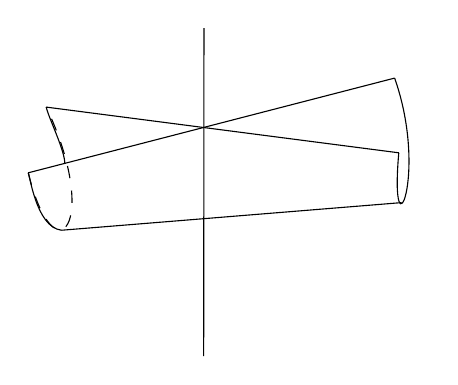
\begin{tikzpicture}[x=0.75pt,y=0.75pt,yscale=-1,xscale=1]
%uncomment if require: \path (0,300); %set diagram left start at 0, and has height of 300

%Straight Lines [id:da3051212884747203] 
\draw    (116.83,167.61) -- (293.36,121.97) ;
%Straight Lines [id:da5970026463866993] 
\draw    (125.5,135.95) -- (295.36,157.97) ;
%Curve Lines [id:da7682892169827296] 
\draw  [dash pattern={on 4.5pt off 4.5pt}]  (116.83,167.61) .. controls (129.47,219.22) and (152.16,191.95) .. (125.5,135.95) ;
%Curve Lines [id:da5380894940965806] 
\draw    (295.36,157.97) .. controls (290.69,210.64) and (310.03,169.3) .. (293.36,121.97) ;
%Straight Lines [id:da7220319461659055] 
\draw    (132.83,195.28) -- (296.69,181.97) ;
%Straight Lines [id:da24050677405998733] 
\draw    (201.5,97.95) -- (201.36,255.97) ;
%Curve Lines [id:da2766589837075546] 
\draw    (116.83,167.61) .. controls (117.47,167.72) and (120.47,193.72) .. (132.83,195.28) ;
%Curve Lines [id:da3571003825201615] 
\draw    (125.5,135.95) .. controls (126.47,140.72) and (134.47,156.72) .. (134.47,163.22) ;





\end{tikzpicture}
\caption{\textcolor{darkcerulean}{Whitney's Umbrella}}
\end{figure}

\noindent \textbf{WARNING !} Any stratification may not be Whitney Stratification. The following is the example for that and it will also prove that condition (a) do not implies condition (b).

\vspace*{0.3cm}

\noindent \examp{5.6} $X = V(x^4+y^4-xyz)$. This variety also have singularity along whole $z$-axis. If we take the startification $X_0 = \emptyset$, $X_1= \qty{z-\text{axis}}$ and $X_2 =X$. Here, there are two strata, $S_{\beta} = X_1$ and $S_{\alpha} = X \setminus X_1$. This satisfies the condition (a) but fails to satisfy condition (b).

\begin{figure}[htbp]
    \centering
    \includegraphics[width = 4.5cm]{image.png}
     \caption{\textcolor{darkcerulean}{Condition (b) fails}}
\end{figure}

\noindent To obtain a Whitney stratification we take $X_0 =\qty{c}$ and rests are as previous. The next two theorems will conclude that any quasi projective variety is a pseudomanifold.

\begin{Thm}{\cite{whit_1965} Whitney}{}
    Any quasi projective variety of pure dimension $n$ has a Whitney startification.
\end{Thm}

\begin{Thm}{\cite{borelintersection} Borel}{}
    Any Whitney startification, $$X=X_n\supseteq X_{n-1}\supseteq \cdots \supseteq X_0$$ of complex quasi projective variety of pure dimension $n$ makes $X$ into a topological pseudomanifold of dimension $2n$ with filtration, $$X=Y_{2n}\supseteq Y_{2n-1}\supseteq \cdots \supseteq Y_0$$ defined by $Y_{2j}=Y_{2j+1}=X_j$
\end{Thm}

\subsection{Normalisations}

For the computational purpose we have defined normalisation of psudomanifold and we have seen there is an isomorphism between the intersection homology groups of the space and the normalised space. Now we will talk about normalizsation of algbraic variety. 

\begin{Def}{(Normal variety) }{}
    A quasi-projective complex variety $X$ is called normal if the stalk at $x$ of the sheaf of regular functions on $X$ is an integrally closed ring for every $x \in X$. i.e. local ring $\mathscr{O}_{X,x} \hookrightarrow k(X)$ is integrally closed.
\end{Def}
\noindent It can be shown using Zariski's Main Theorem (\cite{hartshorne2013algebraic}, Ch. V Thm. 5.2) that if a quasi-projective complex variety $X$ is normal in the algebraic sense then it is topologically normal.

\vspace*{0.2cm}

\noindent Any quasi-projective variety $X$ has a normalisation $\pi: \tilde{X} \rightarrow X$. Here $\tilde{X}$ is a normal quasi-projective variety and $\pi$ is a finite-to-one surjective-holomorphic map (with a suitable universal property) which restricts to an isomorphism over the non-singular part $X_{\text {nonsing }}$ of $X$. (Resolving singularity of $\codim \geq 2$)

\vspace*{0.2cm} 

\noindent The normalisation $\tilde{X}$ of a curve $X$ is always non-singular (Hartshorne [79, Ch. III Ex. 5.8]), and hence by results from previous lecture we have,
$$
I H_i(X) \cong H_i(\tilde{X}) .
$$

In general this does not hold for higher-dimensional varieties since the normalisation need not be non-singular.

\subsection{The Kähler package}

We noted in lecture-1 that the intersection homology of a complex projective variety satisfies a set of theorems collectively termed the Kähler package

\begin{itemize}
    \item[] \textbf{Lefschetz hyperplane theorem.} Following the idea of Deligne there is a proof using Morse theory and sheaf theory. This proof holds for a wider range of perversities than middle. Precisely, \textit{ Let $X$ be an $n$-dimensional complex projective variety, $H$ a hyperplane which is transverse to the strata of some Whitney stratification of $X$, and $p$ a perversity for which $p(c) \leq c$ for all $c$. Then the map $$
    I^p H_i(X \cap H) \rightarrow I^p H_i(X)
    $$
    is an isomorphism for $i<n-1$ and a surjection for $i=n-1$}
    \item Some interesting consequences for a normal complex projective variety $X$.
    \begin{itemize}
        \item[(a)] Take $p$ to be the zero perversity. Using last Proposition of lecture-3 we can deduce that the natural map
        $$
        H^i(X \cap H) \rightarrow H^{i+2}(X)
        $$
        is an isomorphism for $i>n-1$ and surjective for $i=n-1$. 
        \item[(b)] We can show that $I H_1(X) \cong H_1(X)$. By repeatedly applying the Lefschetz hyperplane theorem we deduce that $I H_1(X)$ is isomorphic to the first intersection homology of a surface $Y$ with isolated singularities. Direct computation shows that this group is $H_1(X)$, has even dimension.
    \end{itemize}
 \item[] \textbf{Hard Lefschetz Theorem.} The hard Lefschetz theorem states that multiplication by the Euler class of $E$ induces a map
 $$
 L: I H^i(X) \rightarrow I H^{i+2}(X)
 $$
 which is injective for $i<n$, surjective for $i+2>n$ and such that
 $$
 L^i: I H^{n-i}(X) \rightarrow I H^{n+i}(X)
 $$ is isomorphism for $i \geq 0$.
 \item There are many interesting consequences of this theorem. One simple exmaple is given below - Suppose $X$ is an $n$-dimensional complex projective variety in $\mathbb{C P}^N$ and that $Y$ is the complex cone on $X$, i.e. $Y$ is the affine variety in $\mathbb{C}^{N+1}$ cut-out by the homogeneous polynomials in $N+1$ variables which define $X$. Let $E$ be the tautological line bundle on $X$ whose fibre over $x \in X$ is the line in $\mathbb{C}^{N+1}$ represented by the point $x \in \mathbb{C P}^N$.

 \item[] The vertex $\{0\}$ of the complex cone is a singularity of real codimension $2(n+1)$ and so
 $$
 I H^i(Y)=\left\{\begin{array}{cl}
 I H^i(Y-\{0\}) & i \leq n \\
 0 & \text { otherwise. }
 \end{array}\right.
 $$
 \noindent We have a rank $1$ complex vector bundle, which is therefor $2$-dimensional. Thus there is a `Thom isomorphism' says for any orientated dimension $n$ (in this case $n=2$) vector bundle there is an isomorphism $$T: IH^k(X) \rightarrow IH^ {k+n}(E, E\setminus X)$$ We have LES of cohomology for pair $(E,E\setminus X)$as follows - $$\cdots \rightarrow IH^{i-1}(E \setminus X) \rightarrow IH^i(E, E\setminus X) \rightarrow IH^i(E) \rightarrow IH^i(E\setminus X) \rightarrow \cdots $$
It can be shown that $\pi^{\ast}: IH^{i}(X)\to IH^{i}(E)$ is an isomorphism (using stratified homotopy invariance property). It can be shown the square in the following diagram commutes, \[\begin{tikzcd}
    \cdots & {IH^{i-1}(E\setminus X)} & {IH^{i}(E,E\setminus X)} & {IH^{i-1}(E)} & {IH^{i}(E\setminus X)} & \cdots \\
    && {IH^{i-2}(X)} & {IH^{i}(X)}
    \arrow[from=1-1, to=1-2]
    \arrow[from=1-2, to=1-3]
    \arrow[from=1-3, to=1-4]
    \arrow[from=1-4, to=1-5]
    \arrow[from=1-5, to=1-6]
    \arrow["{\smile e(E)}", color={rgb,255:red,92;green,92;blue,214}, from=2-3, to=2-4]
    \arrow["{\pi^{\ast}}"', color={rgb,255:red,92;green,92;blue,214}, from=2-4, to=1-4]
    \arrow["T", color={rgb,255:red,92;green,92;blue,214}, from=2-3, to=1-3]
    \arrow[color={rgb,255:red,214;green,92;blue,92}, from=1-2, to=2-3]
    \arrow[color={rgb,255:red,214;green,92;blue,92}, from=2-4, to=1-5]
    \end{tikzcd}\]
    and thus we have a LES, \[\begin{tikzcd}
        \cdots & {IH^{i-1}(E\setminus X)} & {IH^{i-2}(X)} & {IH^{i}(X)} & {IH^{i}(E\setminus X)} & \cdots
        \arrow[from=1-1, to=1-2]
        \arrow[from=1-5, to=1-6]
        \arrow[color={rgb,255:red,214;green,92;blue,92}, from=1-2, to=1-3]
        \arrow[color={rgb,255:red,214;green,92;blue,92}, from=1-4, to=1-5]
        \arrow["{\smile e(E)}", color={rgb,255:red,92;green,92;blue,214}, from=1-3, to=1-4]
        \end{tikzcd}\]
        The LES corresponds to of SES (using Hard Lefschetz) $$0\to IH^{i-2}(X)\xrightarrow{\smile e(E)}IH^{i}(X) \to IH^{i}(E\setminus X)\to 0$$ for $i \leq n$. Now note that $Y \setminus \qty{0}$ and $E \setminus X$ are naturally isomorphic. So we have for $i \leq n$, $$IH^i(Y)\simeq IH^{i}(E\setminus X) \simeq IH^{i}(X)/\operatorname{Im} L \simeq IH^{i}_{\text{prim}}(X)$$ where $IH^{i}_{\text{prim}}(X)$ is primitive part of $IH^{i}(X)$, that is not multiple of $e(E)$.
\end{itemize} \textsc{Remark:} \textit{$E$ can be viewed as blow up of $Y$ at origin. The above method will be helpful to compute intersection Homology of a space we get by doing successive blow-ups.}



%%%%%%%%%%%%%%%%%%%




  \printbibliography[ 
        heading=bibintoc,
        title={Bibliography}
    ]

\end{document} 